\chapter{Конструкторский раздел}

\section{Общая структура системы}
Каждый пользователь может как создавать тесты, так и проходить их. Следовательно, могут быть выделены две роли: администратор и испытуемый. Диаграмма вариантов использования представлена на рисунке (\ref{uc:1}).

Система предполагает регистрацию и авторизацию пользователей, создание и прохождение тестов. 
	
Для регистрации пользователю необходимо ввести логин, пароль и электронную почту. Регистрация пройдет успешно в случае, если введенные логин и электронная почта не использованы ранее. В случае успеха, будет создан новый аккаунт и пользователь сразу получит к нему доступ, иначе -- сообщение об ошибке. Диаграмма данного процесса представлена на рисунках (\ref{idef0:00}) -- (\ref{idef0:01}).

Для авторизации пользователь должен ввести свой логин и пароль. Если данные верные, пользователь получит доступ к своему аккаунту, иначе -- сообщение об ошибке. Диаграмма процесса авторизации представлена на рисунках (\ref{idef0:10}) -- (\ref{idef0:11}).

Чтобы создать новый тест, пользователю необходимо ввести название теста и его описание. Далее предоставляется ввод вопросов. После того, как новый вопрос добавлен, пользователь может добавить следующий. В результате будет получен новый тест. Диаграмма данного процесса представлена на рисунках  (\ref{idef0:20}) -- (\ref{idef0:21}).

Для прохождения теста, пользователю необходимо ответить на все предложенные вопросы. После заполнения формы, пользователь отправляет ее на сервер для обработки и получает результат. Диаграмма процесса прохождения теста представлена на рисунках  (\ref{idef0:30}) -- (\ref{idef0:31}).


\begin{figure}[ht!]
	\centering{ 
		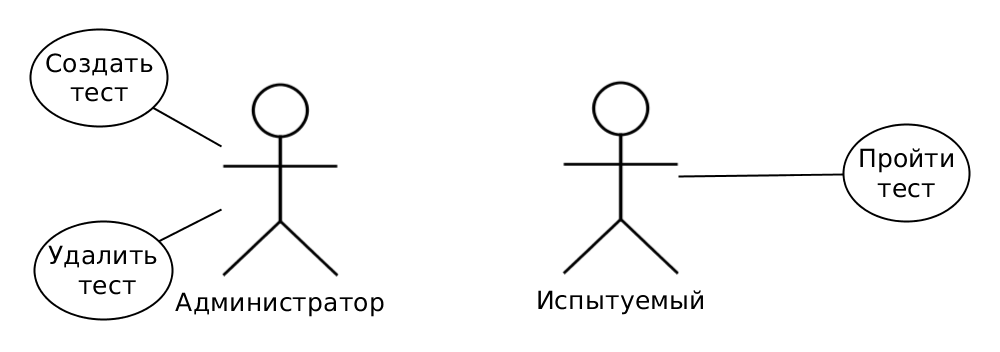
\includegraphics[width=0.8\textwidth]{img/usecase.png}
		\caption{Диаграмма вариантов использования}
		\label{uc:1}}
\end{figure}

\begin{sidewaysfigure}[!ht]
	\centering{ 
		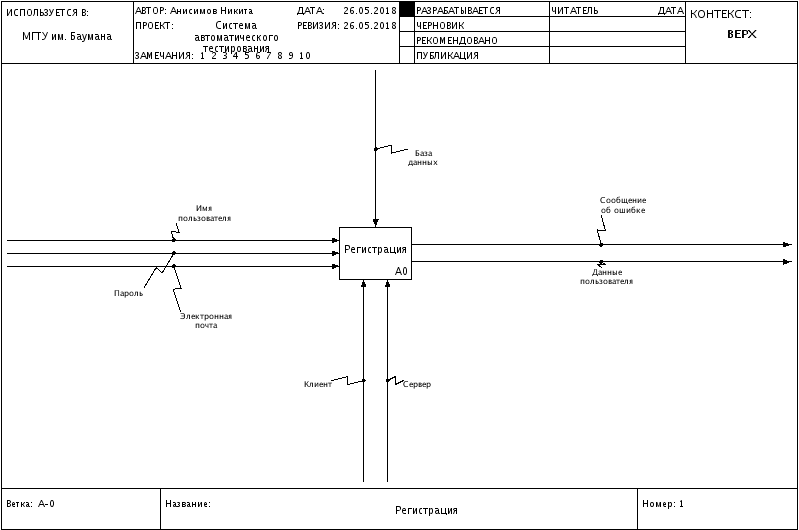
\includegraphics[width=0.8\textwidth]{img/reg_idef/01_A-0.png}
		\caption{Регистрация пользователя (уровень A0)}
		\label{idef0:00}}
\end{sidewaysfigure}
\begin{sidewaysfigure}[!ht]
	\centering{ 
		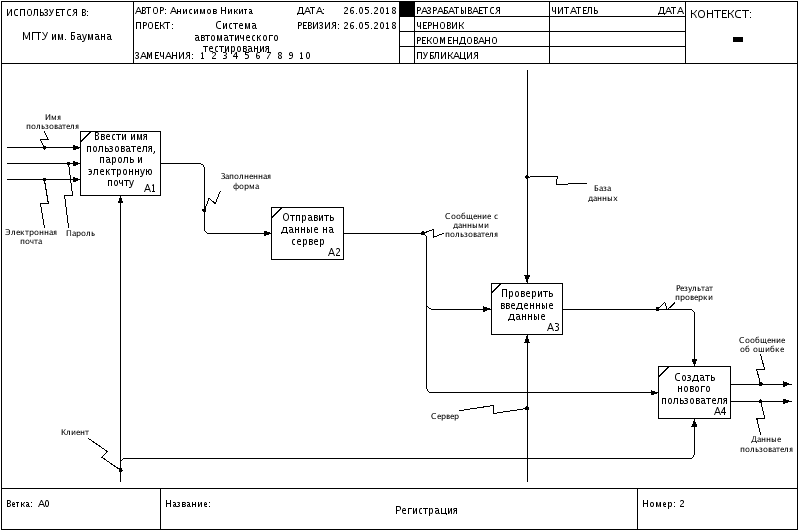
\includegraphics[width=0.8\textwidth]{img/reg_idef/02_A0.png}
		\caption{Регистрация пользователя (ветка А0)}
		\label{idef0:01}}
\end{sidewaysfigure}

\begin{sidewaysfigure}[!ht]
	\centering{ 
		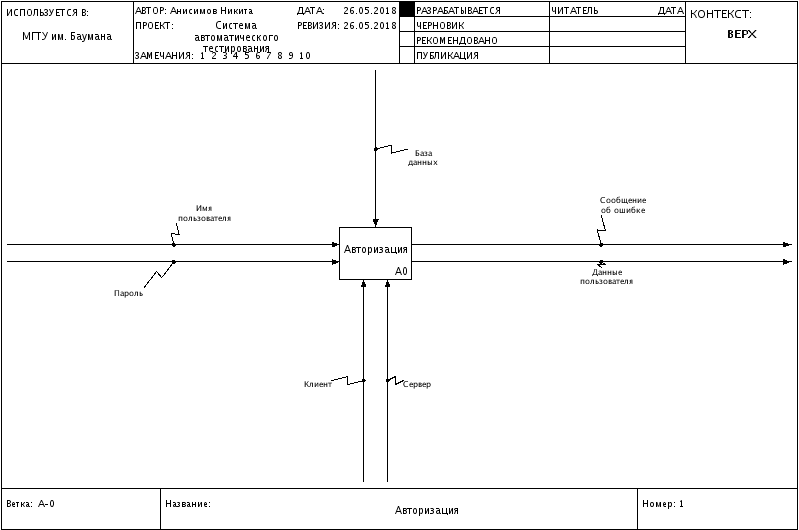
\includegraphics[width=0.8\textwidth]{img/authorzation_idef/01_A-0.png}
		\caption{Авторизация пользователя (уровень A0)}
		\label{idef0:10}}
\end{sidewaysfigure}
\begin{sidewaysfigure}[!ht]
	\centering{ 
		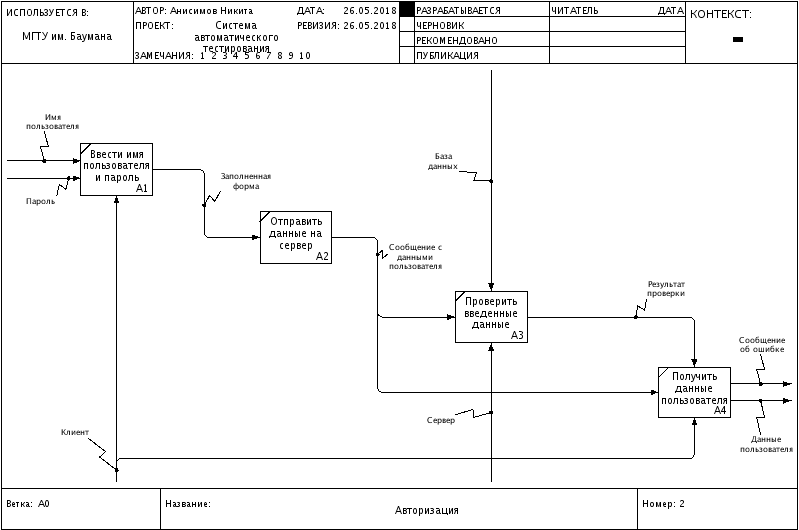
\includegraphics[width=0.8\textwidth]{img/authorzation_idef/02_A0.png}
		\caption{Авторизация пользователя (ветка А0)}
		\label{idef0:11}}
\end{sidewaysfigure}

\begin{sidewaysfigure}[!ht]
	\centering{ 
		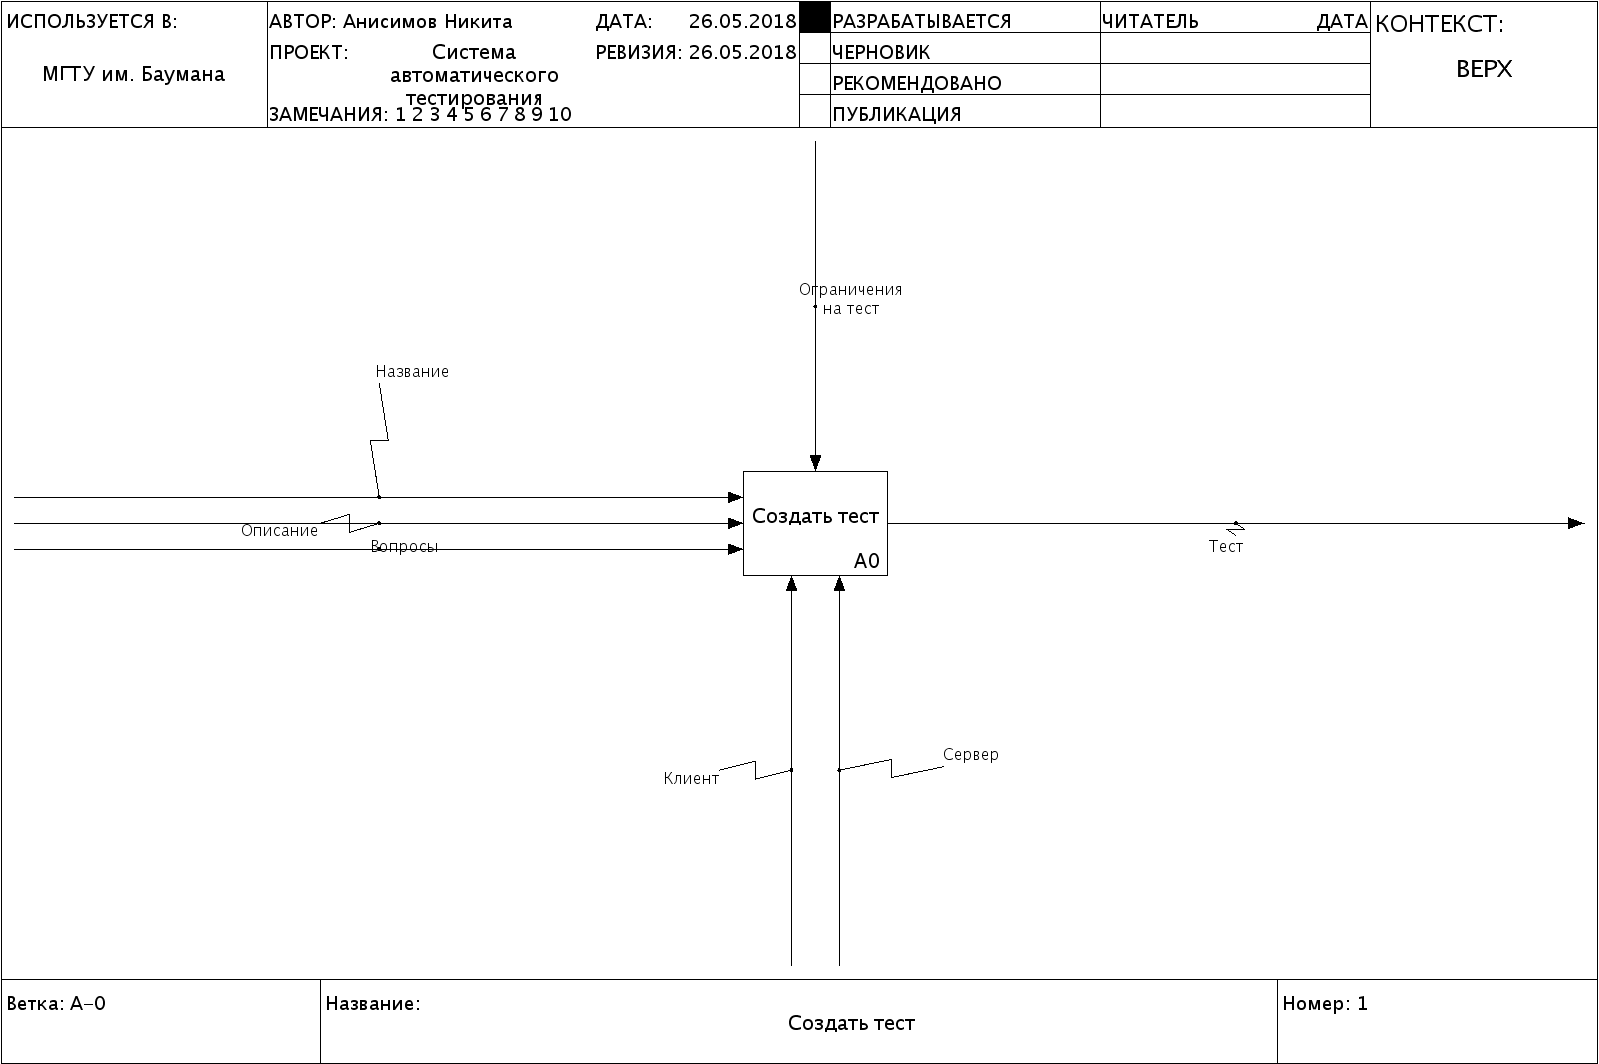
\includegraphics[width=0.8\textwidth]{img/new_idef/01_A-0.png}
		\caption{Создание теста (уровень A0)}
		\label{idef0:20}}
\end{sidewaysfigure}
\begin{sidewaysfigure}[!ht]
	\centering{ 
		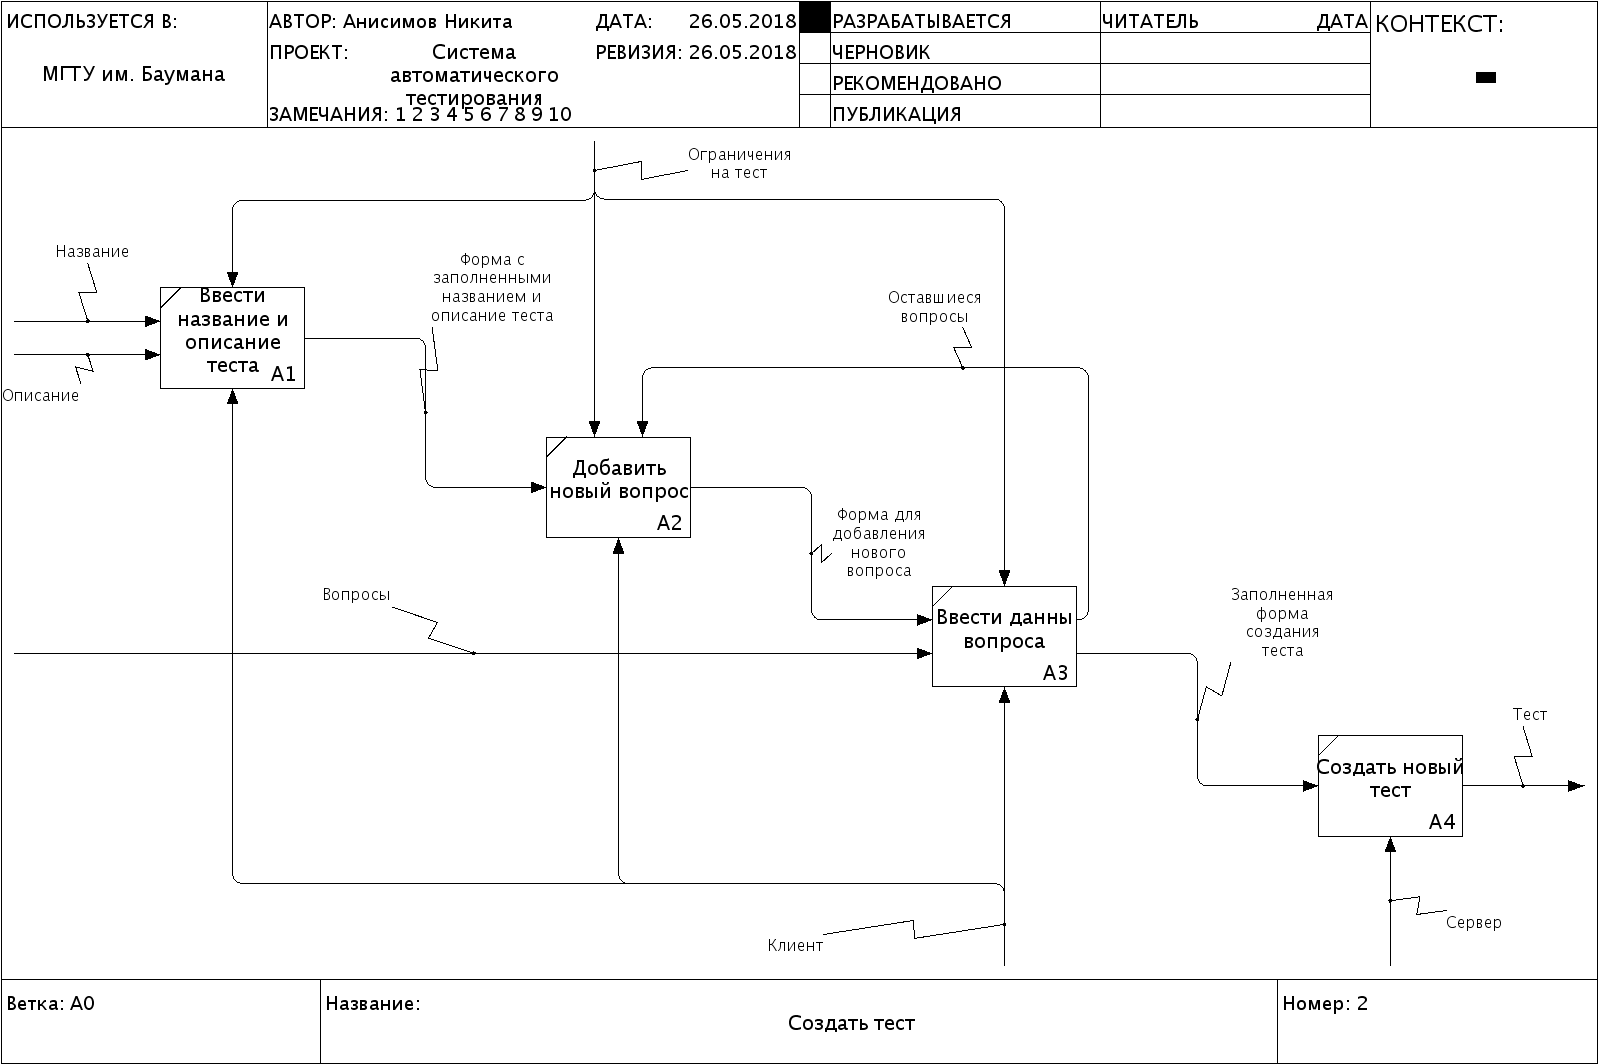
\includegraphics[width=0.8\textwidth]{img/new_idef/02_A0.png}
		\caption{Создание теста (ветка А0)}
		\label{idef0:21}}
\end{sidewaysfigure}


\begin{sidewaysfigure}[!ht]
	\centering{ 
		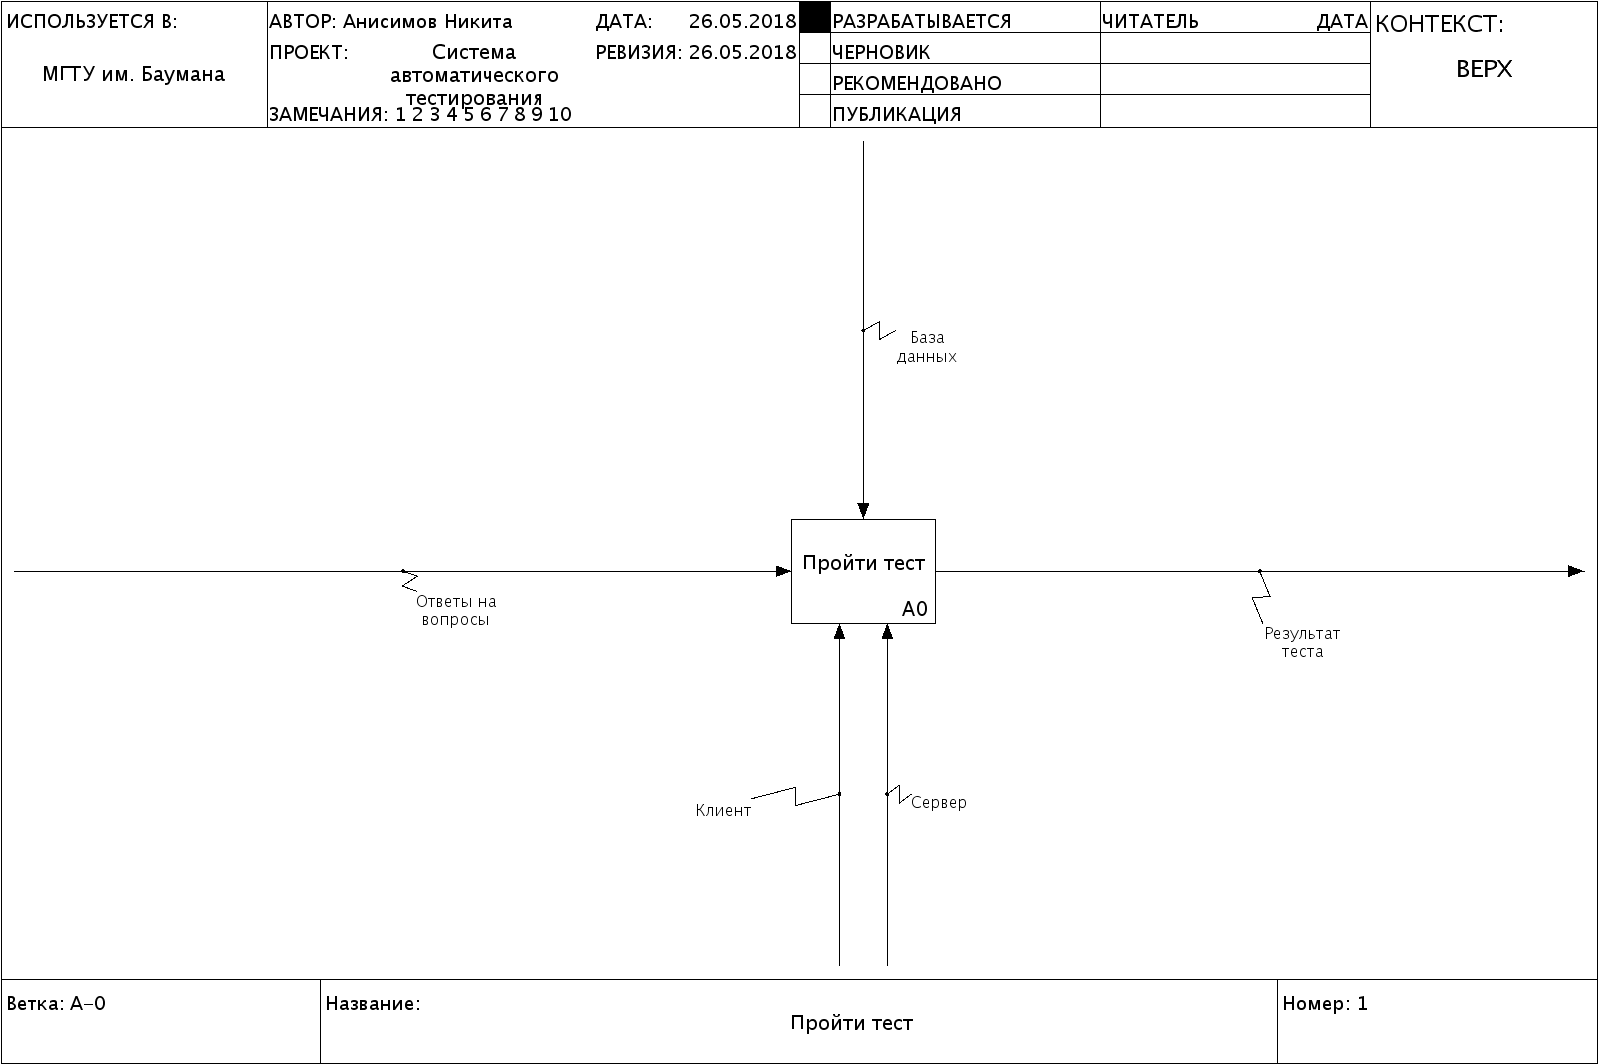
\includegraphics[width=0.8\textwidth]{img/pass_idef/01_A-0.png}
		\caption{Прохождение теста (уровень A0)}
		\label{idef0:30}}
\end{sidewaysfigure}
\begin{sidewaysfigure}[!ht]
	\centering{ 
		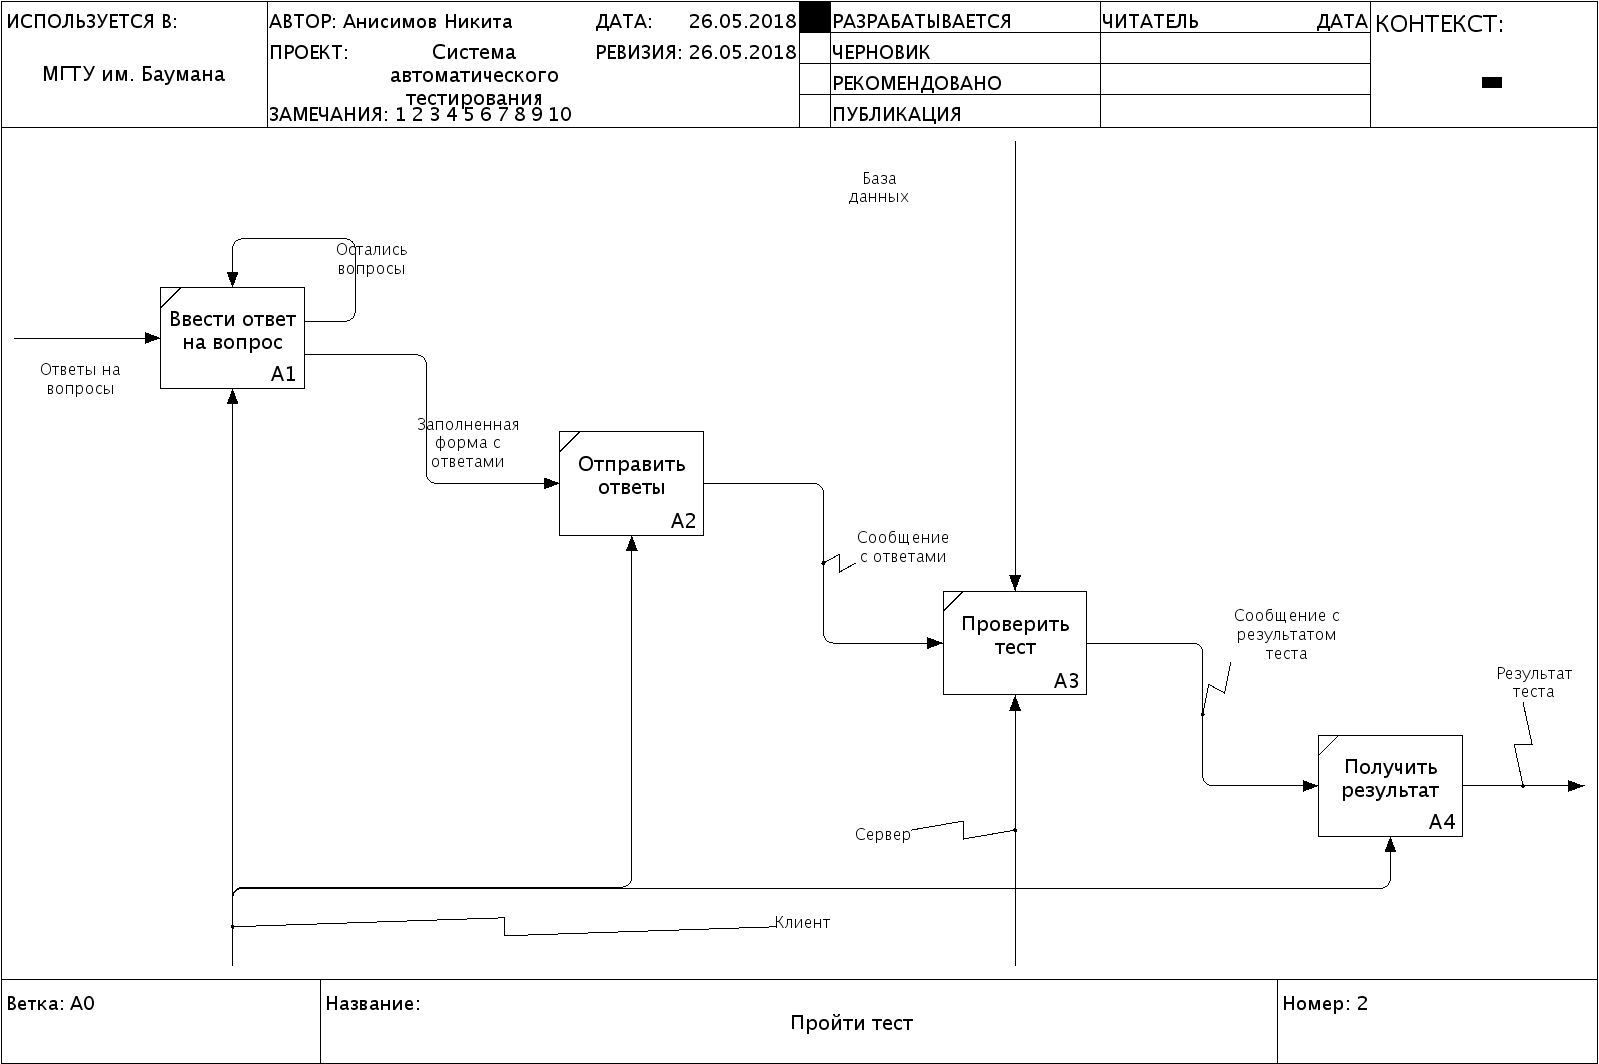
\includegraphics[width=0.8\textwidth]{img/pass_idef/02_A0.png}
		\caption{Прохождение теста (ветка А0)}
		\label{idef0:31}}
\end{sidewaysfigure}


\clearpage
\section{Разработка модели данных}

В результате анализа было выявлено 4 сущности: \texttt{Пользователь}, \texttt{Тест}, \texttt{Результат теста}, \texttt{Вопрос}.
\texttt{Пользователь} может создавать и проходить \texttt{Тесты}. После прохождения \texttt{Теста}, \texttt{Пользователь} получает новый \texttt{Результат теста}. В \texttt{Результате теста} хранится ключ на пройденный \texttt{Тест}. \texttt{Тест} содержит список \texttt{Вопросов}. ER-диаграмма данной модели представлена на рисунке \ref{er:1}.
\begin{figure}[ht!]
	\centering{ 
		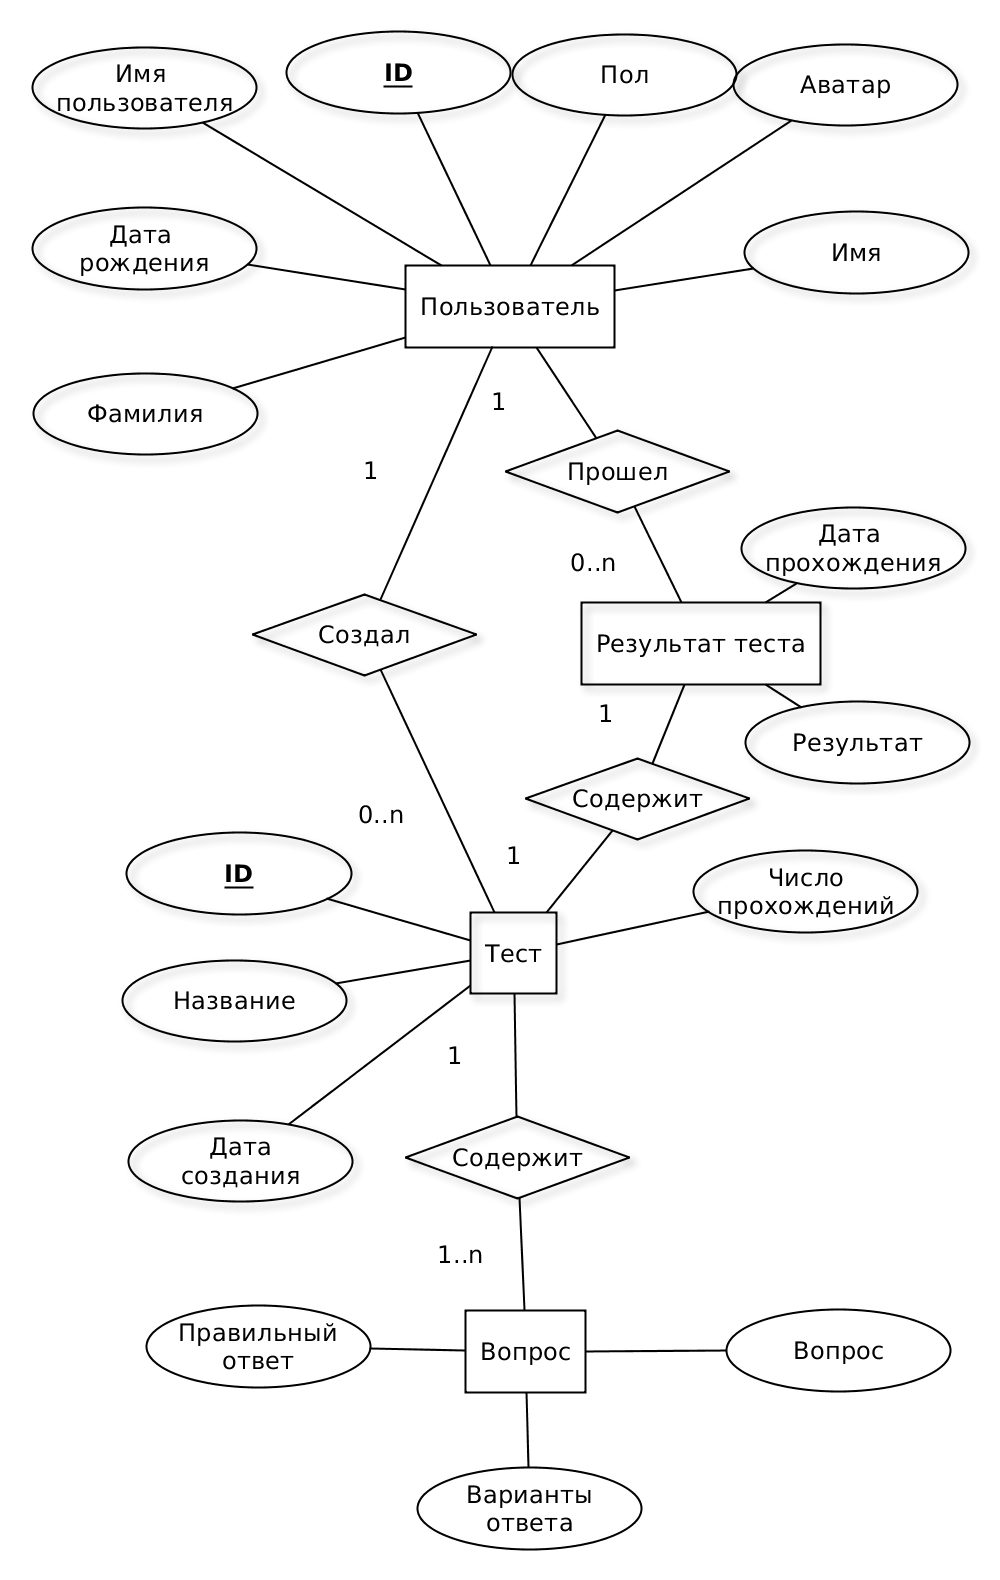
\includegraphics[width=0.7\textwidth]{img/er.png}
		\caption{ER-диаграмма (нотация Чена)}
		\label{er:1}}
\end{figure}

В качестве базы данных выбрана документоориентированная СУБД, благодаря чему становится возможным использование иерархических структур.

В таблицах \ref{user:doc} -- \ref{question:tbl} представлено описание каждой сущности.

\begin{table}[ht!]
	\centering
	\caption{Пользователь}
	\label{user:doc}
	\begin{tabular}{|l|l|l|}
		\hline
		\textbf{Поле} & \textbf{Тип}            & \textbf{Описание}                                                                                                                      \\ \hline
		username      &  Строка               & имя пользователя, уникально, не пусто                                                                                                             \\ \hline
		email         &  Строка               & электронная почта, уникально, не пусто                                                                                                            \\ \hline
		password      &  Строка               & \begin{tabular}[c]{@{}l@{}}пароль, не пусто, \\ не менее 8 символов\end{tabular}                                                       \\ \hline
		avatar        &  Строка               & \begin{tabular}[c]{@{}l@{}}путь до аватара пользователя, не пусто,\\ если аватара нет, путь до стандартного\\ изображения\end{tabular} \\ \hline
		first name    &  Строка               & имя, может быть пусто                                                                                                                  \\ \hline
		second name   &  Строка               & фамилия, может быть пусто                                                                                                              \\ \hline
		birthday      & Дата                    & \begin{tabular}[c]{@{}l@{}}дата рождения, может быть пусто,\\ не может быть больше сегодняшнего дня\end{tabular}                  \\ \hline
		gender        & Пол                     & пол, может быть пусто                                                                                                                  \\ \hline
		passed quiz   & Список<Тест>            & список тестов, может быть пусто                                                                                                        \\ \hline
		created quiz  & Список<Идентификатор>   & \begin{tabular}[c]{@{}l@{}}список ссылок на созданные тестов,\\ может быть пусто\end{tabular}                                          \\ \hline
	\end{tabular}
\end{table}

\begin{table}[ht!]
	\centering
	\caption{Результат теста}
	\label{quizResult:tbl}
	\begin{tabular}{|l|l|l|}
		\hline
		\textbf{Поле} & \textbf{Тип}  & \textbf{Описание}                   \\ \hline
		quiz id       & Идентификатор & ссылка на пройденный тест, не пусто \\ \hline
		result        &  Строка     & результат теста, не пусто           \\ \hline
		passing date  & Дата          & дата прохождения теста, не пусто    \\ \hline
	\end{tabular}
\end{table}

\begin{table}[ht!]
	\centering
	\caption{Тест}
	\label{quiz:tbl}
	\begin{tabular}{|l|l|l|}
		\hline
		\textbf{Поле}  & \textbf{Тип}   & \textbf{Описание}                \\ \hline
		name           &  Строка      & название теста, не пусто         \\ \hline
		description    &  Строка      & описание теста, не пусто         \\ \hline
		creation date  & Дата           & дата прохождения теста, не пусто \\ \hline
		passing number & Целое          & число сдач теста, не пусто       \\ \hline
		question       & Список<Вопрос> & список вопрос, не пусто          \\ \hline
	\end{tabular}
\end{table}

\begin{table}[ht!]
	\centering
	\caption{Вопрос}
	\label{question:tbl}
	\begin{tabular}{|l|l|l|}
		\hline
		\textbf{Поле} & \textbf{Тип}   & \textbf{Описание}                   \\ \hline
		text          &  Строка      & текст вопроса, не пусто             \\ \hline
		answer        &  Строка      & правильный вариант ответа, не пусто \\ \hline
		variants      & Список<Строка> & список вариантов ответа, не пусто   \\ \hline
	\end{tabular}
\end{table}

\section{Взаимодействие компонентов системы}

Взаимодействие компонентов системы представлено при помощи диаграмм последовательностей, изображенных на рисунках (\ref{seq:1}) -- (\ref{seq:10}). 

\begin{figure}[ht!]
	\centering{ 
		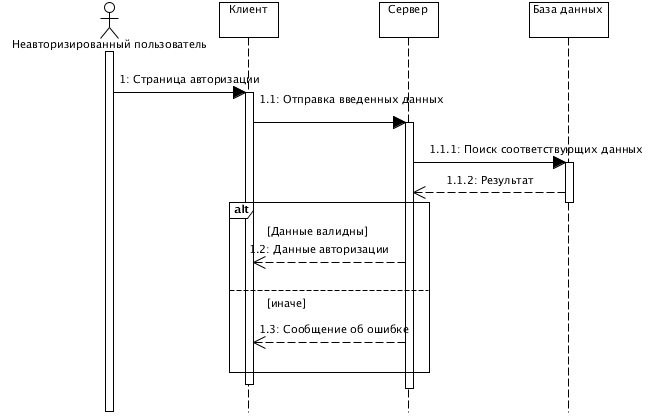
\includegraphics[width=1\textwidth]{img/sequence1.png}
		\caption{Взаимодействие компонентов при авторизации пользователей}
		\label{seq:1}}
\end{figure}
\begin{figure}[ht!]
	\centering{ 
		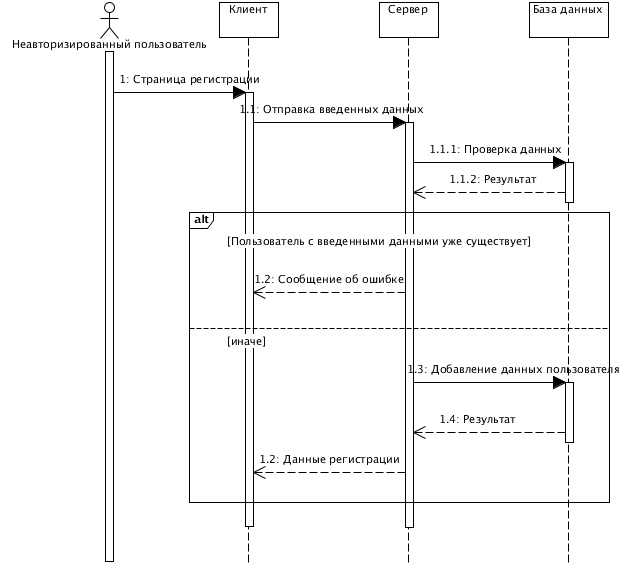
\includegraphics[width=1\textwidth]{img/sequence2.png}
		\caption{Взаимодействие компонентов при регистрации пользователей}
		\label{seq:2}}
\end{figure}
\begin{figure}[ht!]
\centering{ 
	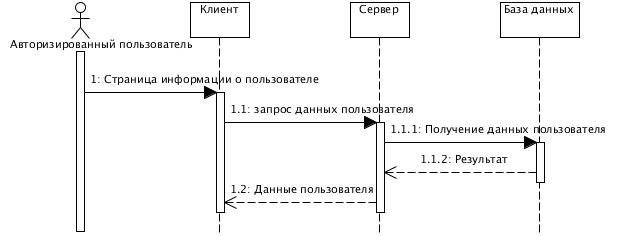
\includegraphics[width=1\textwidth]{img/sequence3.png}
	\caption{Взаимодействие компонентов при запросе данных пользователя}
	\label{seq:3}}
\end{figure}
\begin{figure}[ht!]
\centering{ 
	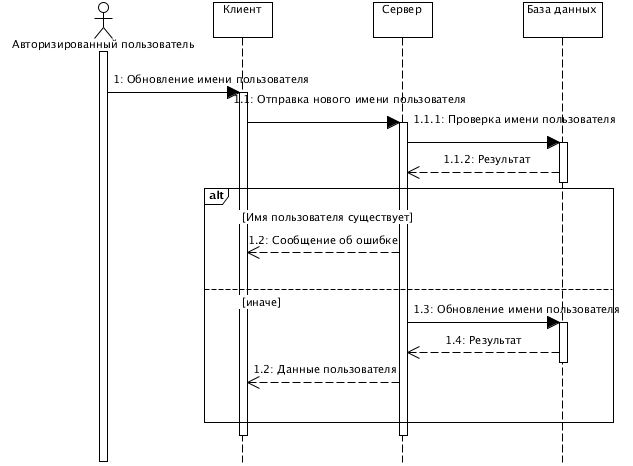
\includegraphics[width=1\textwidth]{img/sequence4.png}
	\caption{Взаимодействие компонентов при изменении имени пользователя}
	\label{seq:4}}
\end{figure}
\begin{figure}[ht!]
\centering{ 
	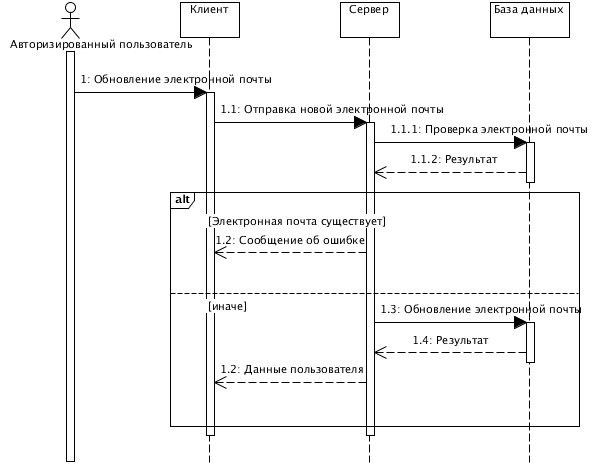
\includegraphics[width=1\textwidth]{img/sequence5.png}
	\caption{Взаимодействие компонентов при изменении электронной почты}
	\label{seq:5}}
\end{figure}
\begin{figure}[ht!]
\centering{ 
	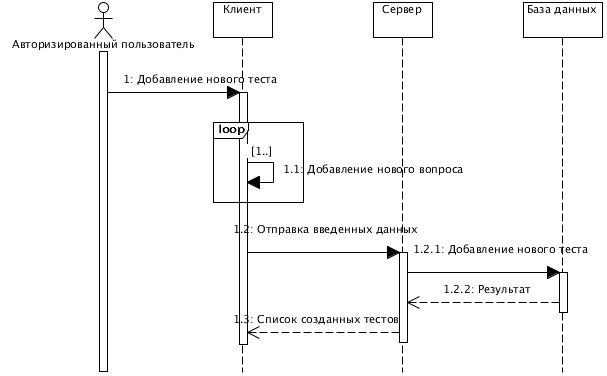
\includegraphics[width=1\textwidth]{img/sequence6.png}
	\caption{Взаимодействие компонентов при добавлении нового теста}
	\label{seq:6}}
\end{figure}
\begin{figure}[ht!]
	
\centering{ 
	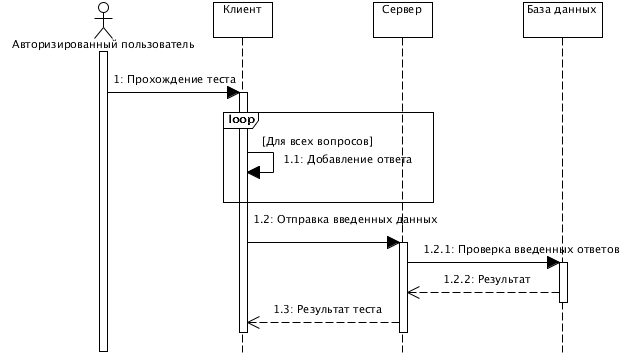
\includegraphics[width=1\textwidth]{img/sequence7.png}
	\caption{Взаимодействие компонентов при прохождении теста}
	\label{seq:7}}
\end{figure}
\begin{figure}[ht!]
\centering{ 
	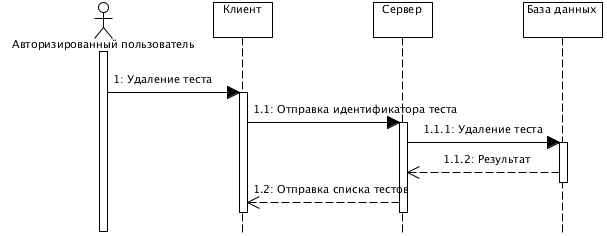
\includegraphics[width=1\textwidth]{img/sequence8.png}
	\caption{Взаимодействие компонентов при удалении теста}
	\label{seq:8}}
\end{figure}
\begin{figure}[ht!]
\centering{ 
	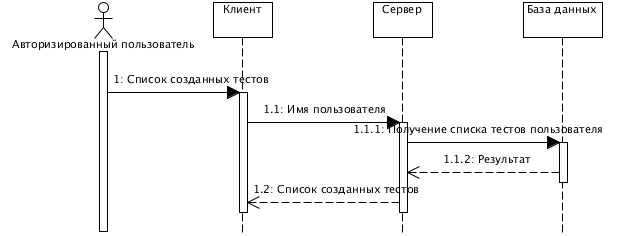
\includegraphics[width=1\textwidth]{img/sequence9.png}
	\caption{Взаимодействие компонентов при получении списка созданных пользователем тестов}
	\label{seq:9}}
\end{figure}
\begin{figure}[ht!]
\centering{ 
	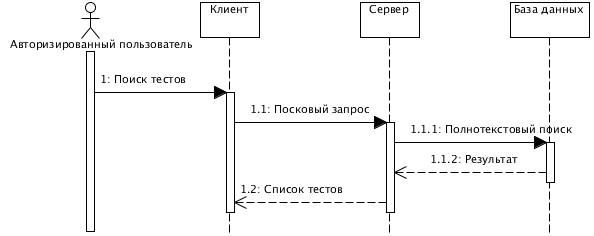
\includegraphics[width=1\textwidth]{img/sequence10.png}
	\caption{Взаимодействие компонентов при поиске тестов}
	\label{seq:10}}
\end{figure}

\clearpage
\section{Вывод}
Разрабатываемая система предназначена для проведения автоматического тестирования пользователей. Были определены две роли: администратор, испытуемый. 

Процессы авторизации, регистрации, добавления и прохождения тестов детально документированы при помощи IDEF0 диаграмм.

В ходе анализа выявлены следующие сущности: \texttt{Пользователь}, \texttt{Тест}, \texttt{Результат теста}, \texttt{Вопрос}. Каждая сущность описана и документирована. Была построена ER-диаграмма для данного набора сущностей.   

Определены варианты взаимодействия подсистем для следующих действий: авторизация, регистрация, запрос данных пользователя, изменение имени пользователя, изменение пароля пользователя, изменение электронной почты пользователя, добавление нового теста, прохождение теста, удаление теста, получение списка созданных тестов, поиск тестов.

